\section{Artificial Intelligence}
\subsection{overview} 
        after breaking the Enigma machine that was made by the Nazies for secure/encrypted communications in world war against the alies, Alan Turing once again changed the course of history by asking the following question "Can machines think?" in a paper he published in 1950 titled "Computing Machinery and Intelligence", this question is what gave rise to Artificial Intelligence, because all what artificial intelligence is trying to do is answer that question in the affirmative by trying to mimic human intelligence in machines ~\cite{ai} to do so Turing has put forward a test called "The Turing Test" which will be explained later , now because artificial intelligence is a concept that is  so broad and general people dont always agree on a definition, but we found that the below definition is a good enough explanation.
        
    \subsection{definition}
        "Artificial intelligence (AI) is a wide-ranging branch of computer science concerned with building smart machines capable of performing tasks that typically require human intelligence." ~\cite{ai}

    \subsection{turing test}
        it is basically a test put forward by the mathematician Alan Turing to determin whether a machine is intteligent or not, the test goes as follows, "If a machine can engage in a conversation with a human without being detected as a machine, it has demonstrated human intelligence." ~\cite{turing}
    
    \subsection{the 4 types of Artificial Intelligence}
        \begin{description} 
        \item[Reactive Machines]
            it is one of the most basic form of artificial intelligence because as the title suggests it only reacts to its surrounding environment, and does not use a memory to try and learn from past experience so it is purely reactive which means that this type of artificial intelligence can only be responsible for a very narrow and spepcialised set of tasks, this narrowness can be looked at as a limitation but in fact it is what makes it special in being very trust worthy and error free. a famous example of this type would be the chess playing machine Deep Blue made by IBM in the 1990's which treats each move in the game as it own seperate reality and doesnt rely on past moves ~\cite{ai}
        \item[Limited Memory]
            it is a type of artificial intelligence that relies on memory and automatic training , which means learning from past experience to try to make optimised decisions/predictions, the learning steps in this type can be looked at as a feedback loop (generate data, learn, make model, make predictions, accept feedback), there are 3 major models that utilise this type ~\cite{ai}: 
                Reinforcement learning
                    learning from trial and error
                Long Short Term Memory (LSTM)
                    uses past data to make predictions, the more recent the data the more weight it has on making predictions
                Evolutionary Generative Adversarial Networks (E-GAN)
                    this model grows constantly by putting 2 machines against each other and they learn by bouncing information off of each other. 
        \item[Theory of Mind]
            this is purely theoretical and technology is still not caught up to this, and it stipulates that machines would be able to understand how humans and animals think and feel and make decisions throught self reflection ~\cite{ai}.
        \item[Self-awareness]
            after Theory of Mind is established this is the next step, where machines bacome self aware and comprehensive of its own existence by obtaining human level intelligence and consciousness ~\cite{ai}.
        \end{description}
    
    \subsection{Artificial Intelligence Categories}
        generally speaking there are 2 categories of artificial intelligence ~\cite{ai}

            \begin{description} 
            \item[Narrow artificial intelligence]
                also know as "Weak artificial intelligence", it operates in a limited context and is often specialised in a single task such as : Google Search, Image Recognition, Self-Driving Cars...etc
            \item[artificial general intelligence]
                also know as "Strong artificial intelligence", it is the kind of artificial intelligence we see in Science Fiction movies implimented in robots that have human level intelligence and that can apply its intelligence to solve any problem.
            \end{description}
\section{Machine Learning}
    \subsection{overview}
        machine learning is a subfield of artificial intelligence that has a human like ability to learn from past experience through statistics and data and it has helped us solve difficult world problems ranging from medical problems to environmental issues, and the special thing about machine learning is its ability to solve these problems wthout being explicitly programmed to do so with the usual sequence of code lines that define normal (non artificial intelligence ) algorithms, but it relies on tacit knowledge (past experience) to try and find patterns and make predictions, humans use tacit knowledge all the time for example a person cant accuratly explain how he preforms face recognition but it is gained through the experience of observing that face numerous times in different angles and states~\cite{ml}

    \subsection{definition}
        "Machine learning is a subset of artificial intelligence that gives systems the ability to learn and optimize processes without having to be consistently programmed. Simply put, machine learning uses data, statistics and trial and error to “learn” a specific task without ever having to be specifically coded for the task."~\cite{ml}

    \subsection{types of machine learning algorithms}
        there are 3 types ~\cite{ml}
        \begin{description}
        \item[Supervised Learning]
            supervised machine learning algorithms provide a mathematical model that can make the connection between inputs and outputs of the training data (pre-labeled data) in the most optimised way so that when it is provided with new data it can make vary accurate predictions. regression and classification are the most popular supervised algorithms 
        \item[Unsupervised Learning]
            Unsupervised algorithms take unlabeled input data and try to structure it in the form of clustering or grouping by taking into account commonaities or lack of commonaities.
        \item[Semi-Supervised Learning]
            this types falls in the middle, it is given labeled and unlabeled data with unlabeled being the bigger percentage then the algorithm is going to cluster the unlabeled data throught the structure of the labeled data which offers a huge optimisation for both sides, because supervised learning requires a huge size of labeled data which is usualy done by human beings which means that it takes alot of time and is bound to human error, and Unsupervised learnning algorithms takes alot of time also figuring out the connections in the raw unlabeled data.
        \end{description}

    \subsection{examples and applications}
        as mentioned in ~\cite{ml}
        \begin{description}
        \item [Financial Services]
            this industry is using machine learning almost in every aspect, because of its ability to speed up the financial processes and preform tasks that used to take humans days or weeks in merely seconds. such as handling millions of transactions, recommending personal offers ... etc
        \item [Healthcare]
            this industry is also relying alot on machine learning because of its ability to discover new treatements and detect and predict diseases, a medical professional equiped with machine learning is far more proficient because he can access a patient's relevant medical history in blink of an eye rather that digging through files or contacting other departements in the hospital. machine learning is predicted to save the medical field billions of dollars annualy
        \item [Social Media]
            this industry usually uses machine learning for 2 main reasons: strengthening the feel of connection between people and iliminating bad actors, it does the former by providing individualised recommendations to friends, pages, and communities based on a user's preference or activity history, and for the latter it tries to prevent fake news before it becomes a thing, block malicious users and scams when detecting abnormalities.

        \item [...etc]
        \end{description}

\section{Deep Learning}
    \subsection{overview}
        yet again another subfield with great capabilities, although it seems to be a new concept but it actually isn't as our professor Rahmoun Abdellatif once mentioned in a lecture talking about deep learning and neural networks, he said that the theoretical part was established along time ago (1950's) but people back then didnt't have the computational power to impliment it, so it took quite some time for people to develop the necessary computational power to take on artificial neural networks and one of the scientists whi made neural networks cool again is Geoffrey Hinton by demonstrating that a few of them could be trained using backprobagation for better shape recognition and word prediction and by 2012 deep learning is basicaly used every where ~\cite{dl}.

    \subsection{definition}
        "Deep learning (sometimes known as deep structured learning) is a subset of machine learning, where machines employ artificial neural networks to process information. Inspired by biological nodes in the human body, deep learning helps computers to quickly recognize and process images and speech. Computers then "learn" what these images or sounds represent and build an enormous database of stored knowledge for future tasks. In essence, deep learning enables computers to do what humans do naturally- learn by immersion and example."~\cite{dl}

    \subsection{what is next?}
        although deep learning has brought us many accomplishements and it can be applied in various domains and when it is done right it can preform a certain task with super-human level but some scientists an researchers say it is only a small step in aquiring actual intelligent machines because it lacks the concept of abstract ideas and knowledge such as: what objects are?, chat they are for?, how to use them?...etc
        and also the problem of "data" because deep learning requires a huge amount of pre labeled data to be trained which is not always available and public datasets wont cut it~\cite{dl}.

        and there are alot of new concepts that are presenting promising results like "deep reinforcement learning" a combination of deep learning and reinforcement learning and we can see this implimented in a software called AlphaGo and AlphaGo Zero, another research paper suggested  "Reward learning from human preferences and demonstrations" which basically means machines learn from observing humans play games which they say it works better then trial-and-error systems~\cite{dl}

        \bigskip \textbf{other ideas that are worth mentioning} ~\cite{dl}
            \begin{description}
            \item [ONE-SHOT LEARNING and NAS (neural architecture search)]
                one-shot learning means we need far less data to learn, and NAS means an algorithm finds the best neural network architecture to solve a problem, this combination is very promising
            \item [GANS (Generative Adversarial Networks)]
                a competition for deep learning which puts 2 networks against each other (a generator and a discriminator) you can think of it as a counterfeiter and a cop.
            \item [AUTOML]
                learn-to-learn which basically means machine learning algorithms do the hard work of finding the design of the network and all we need to provide is data.
            \end{description}


\section{Ai vs Machine Learning vs Deep Learning}
    after all what we have talked about it is obvious that the relationship between the three is an inclusion relationship, deep learning is a subset of machine learning which is a subset of artificial intelligence as shown in Figure ~\ref{fig:versus} 

\begin{figure}[htbp]
\begin{center}
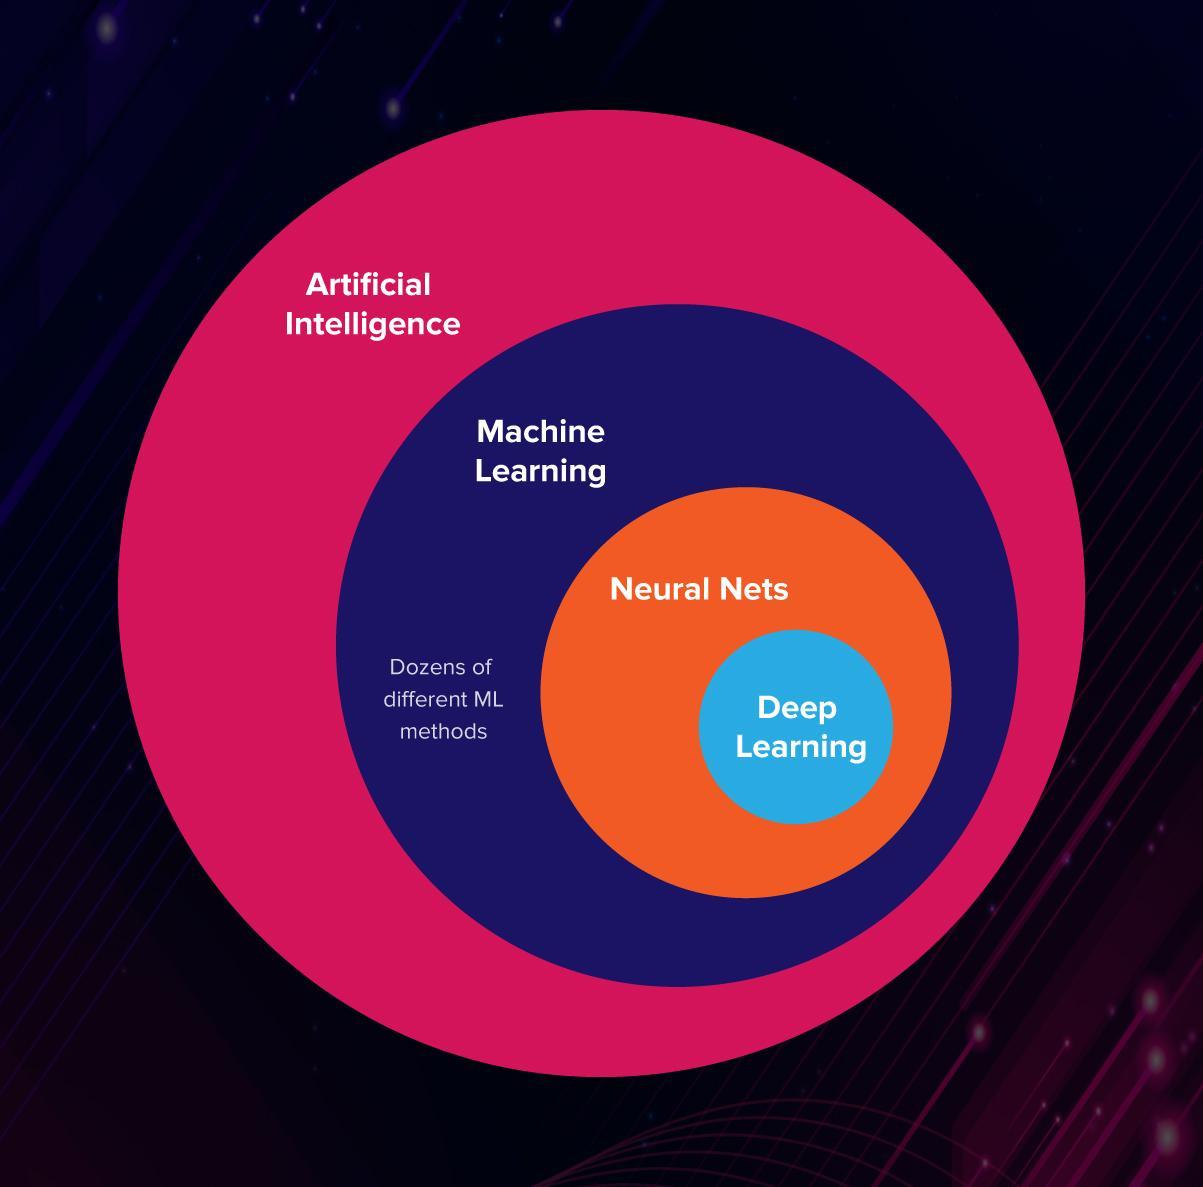
\includegraphics[width=10cm]{./chapter-02-general-ai-information/versus.jpg}
\end{center}
\caption{Skin Anatomy ~\cite{versus}}
\label{fig:versus}
\end{figure}



computer vision
    overview
        yet another subfield of artificial intelligence which is used to train machines to see, and by see we mean process analyse and extract usefull information from images/videos just like us human beings, although our vision is far more advanced in many aspects because our brains were trained since birth to see, analyse objects, understand the distance and relationship between objects, attribute abstract information to objects...etc but it is safe to say that machines can surpass our vision in certain specialised tasks because of there ability to process thousands of images/frames in a short period of time due to the constant increase in computational power especialy (graphical processing). computer vision is used in a wide variety of idustries and its market is estimated to reach 48,6 billion USD by 2022 [ref1]


    using machine learning methods
        in the case of using machine learning for computer vision there are mainly 4 steps to execute, the first step is data preparation (preprocessing) in this step we need to preform some manipulations and transformations to clean the image data, some of these manipulations are cleaning noise, convertion images to the same format, cropping, using gray scale instead of RBG...etc, each case requires its own set of manipulations and transformations. The second step is feature extraction which represents the hard work in most of the cases, in this step we extract a certain set of predefined features to be feeded later to the algorithm, the third step is model training using the prelabeled feature vectors, and the last step is predictions made for new image data, and for this we can chose from a variety of machine learning algorithms depending on our problem: Bayesian Nets, Decision Trees, Nearest Neighbors...etc[ref2]
        ---figure---
    using deep learning 
        applying deep learning in computer vision is totaly different from applying classical machine learning algorithms, firstly,  deep learning requires quantity (huge amounts of image data) over quality to have a robust model with accurate predictions, secondly neural networks saves us the trouble of feature extraction especialy when using Convolution Neural Networks [ref3](Convolution: a mathematical operation on two functions to produce a third function [ref1]) this architecture of neural networks is specialised in processing image data and it is built on three primaty layers Convolution layer, pooling layer and fully connected layer [ref2]

        Convolution layer
            this layer does most of the hard work by identifying and extracting the features, this is done by applying a filter of random size to blocks of the input image using the dot product between matrices
        pooling layer 
            after the feature extraction resulting from the Convolution layer we need to Simplify (by reducing a bloc of values to a single value) the image for easy learning, there are 2 pooling operations max pooling and average pooling 
        fully connected layer
            it operates on a flatened input, where each input is connected to all of the neurons, it is usualy found at the and of the network connecting the hidden layers to the output which help in optimizing the class scores
        ---figure---
    

    applications of computer vision
        there are alot of indsutries using computer vision and these are just a few examples [ref2]
        medical imaging: 
            it helps medical professionals interpret faster and diagnose abnormalities.
        law enforcement en security
            like in surveillance and authentication
        self driving machines like cars and robots
        gaming: augmented reality and virtual reality
        pattern recognition

    some technologies of computer vision
        because of the wide utility of computer vision and its benefits there are alot of libraries and frameworks that facilitates alot of the hard and repeated tasks, here we mention a few of them [ref2]
        openCV 
            a python library for computer vision, 
                super easy to use, 
                a huge library of image processing algorithms, 
                open source, 
                works with GPUs
        Tensorflow
            made by Google and one of the most popular machine learning frameworks 
                with a wide rane of machine/deep learning algorithms, 
                open source, 
                GPU configured
        PyTorch
            made by facebook a neural network framework, 
                used alot by researchers, 
                open source, 
                works with GPUs
        Caffe
            a deep learning framework developed by Berkeley AI Research
                open source
                c++ based 
                easy to use
                fats execution 



